\documentclass{article}
\usepackage{authblk} % Agrega afiliaciones
\usepackage[english]{babel}
\usepackage{hyperref}
\usepackage{float}
\usepackage[utf8]{inputenc} % Forza encoding en utf8
\usepackage{natbib} % Importa bibliografía
\usepackage{caption,ragged2e,tabularx}
\usepackage{graphicx}

\renewcommand{\figurename}{Figura}
%\decimalpoint

\title{Estimation of remaining individuals by area in Socorro Island \\
    \Large{Feral cat eradication project in Socorro Island, Revillagigedo National Park, Mexico}}
\author{Fernando Alvarez}
\author{Maritza Bello}
\author{Braulio Rojas}
\affil{Data Science Direction}

\begin{document}
\maketitle

\begin{abstract}
   According to the data up to August 2019, we determined that: 1) the most probable amount of the remnant cats is 75 individuals; and 2) considering an effort similar to the latest trends and consider an increase rate equal to zero, we will complete eradication in September 2020.
\end{abstract}


\section*{Current status}

Following the methodology proposed by Ramsey (2011) and using data from the feral cat eradication project on Socorro Island until August 2019, we estimate that the initial population size was 841 cats. To date, 766 cats have been removed and the most probable number of remaining individuals is 75 cats. As such, 8 cats must be removed in order to enter the mop-up phase.

\begin{table}[H]
\centering
\caption{\small{Current eradication status}}
\label{table:esfuerzoCapturas}
\begin{tabular}{ |c|c|c| }
    \hline
    Current & Percentage & Cats \\
    \hline
    Initial population size & 100\%    & 841 \\
    Cumulative number of cats removed & 91\%     & 766 \\
    Remaining cats & 9\%     & 76 \\
    \hline
\end{tabular}
\end{table}


\section*{Results}

\begin{figure}[H]
    \centering
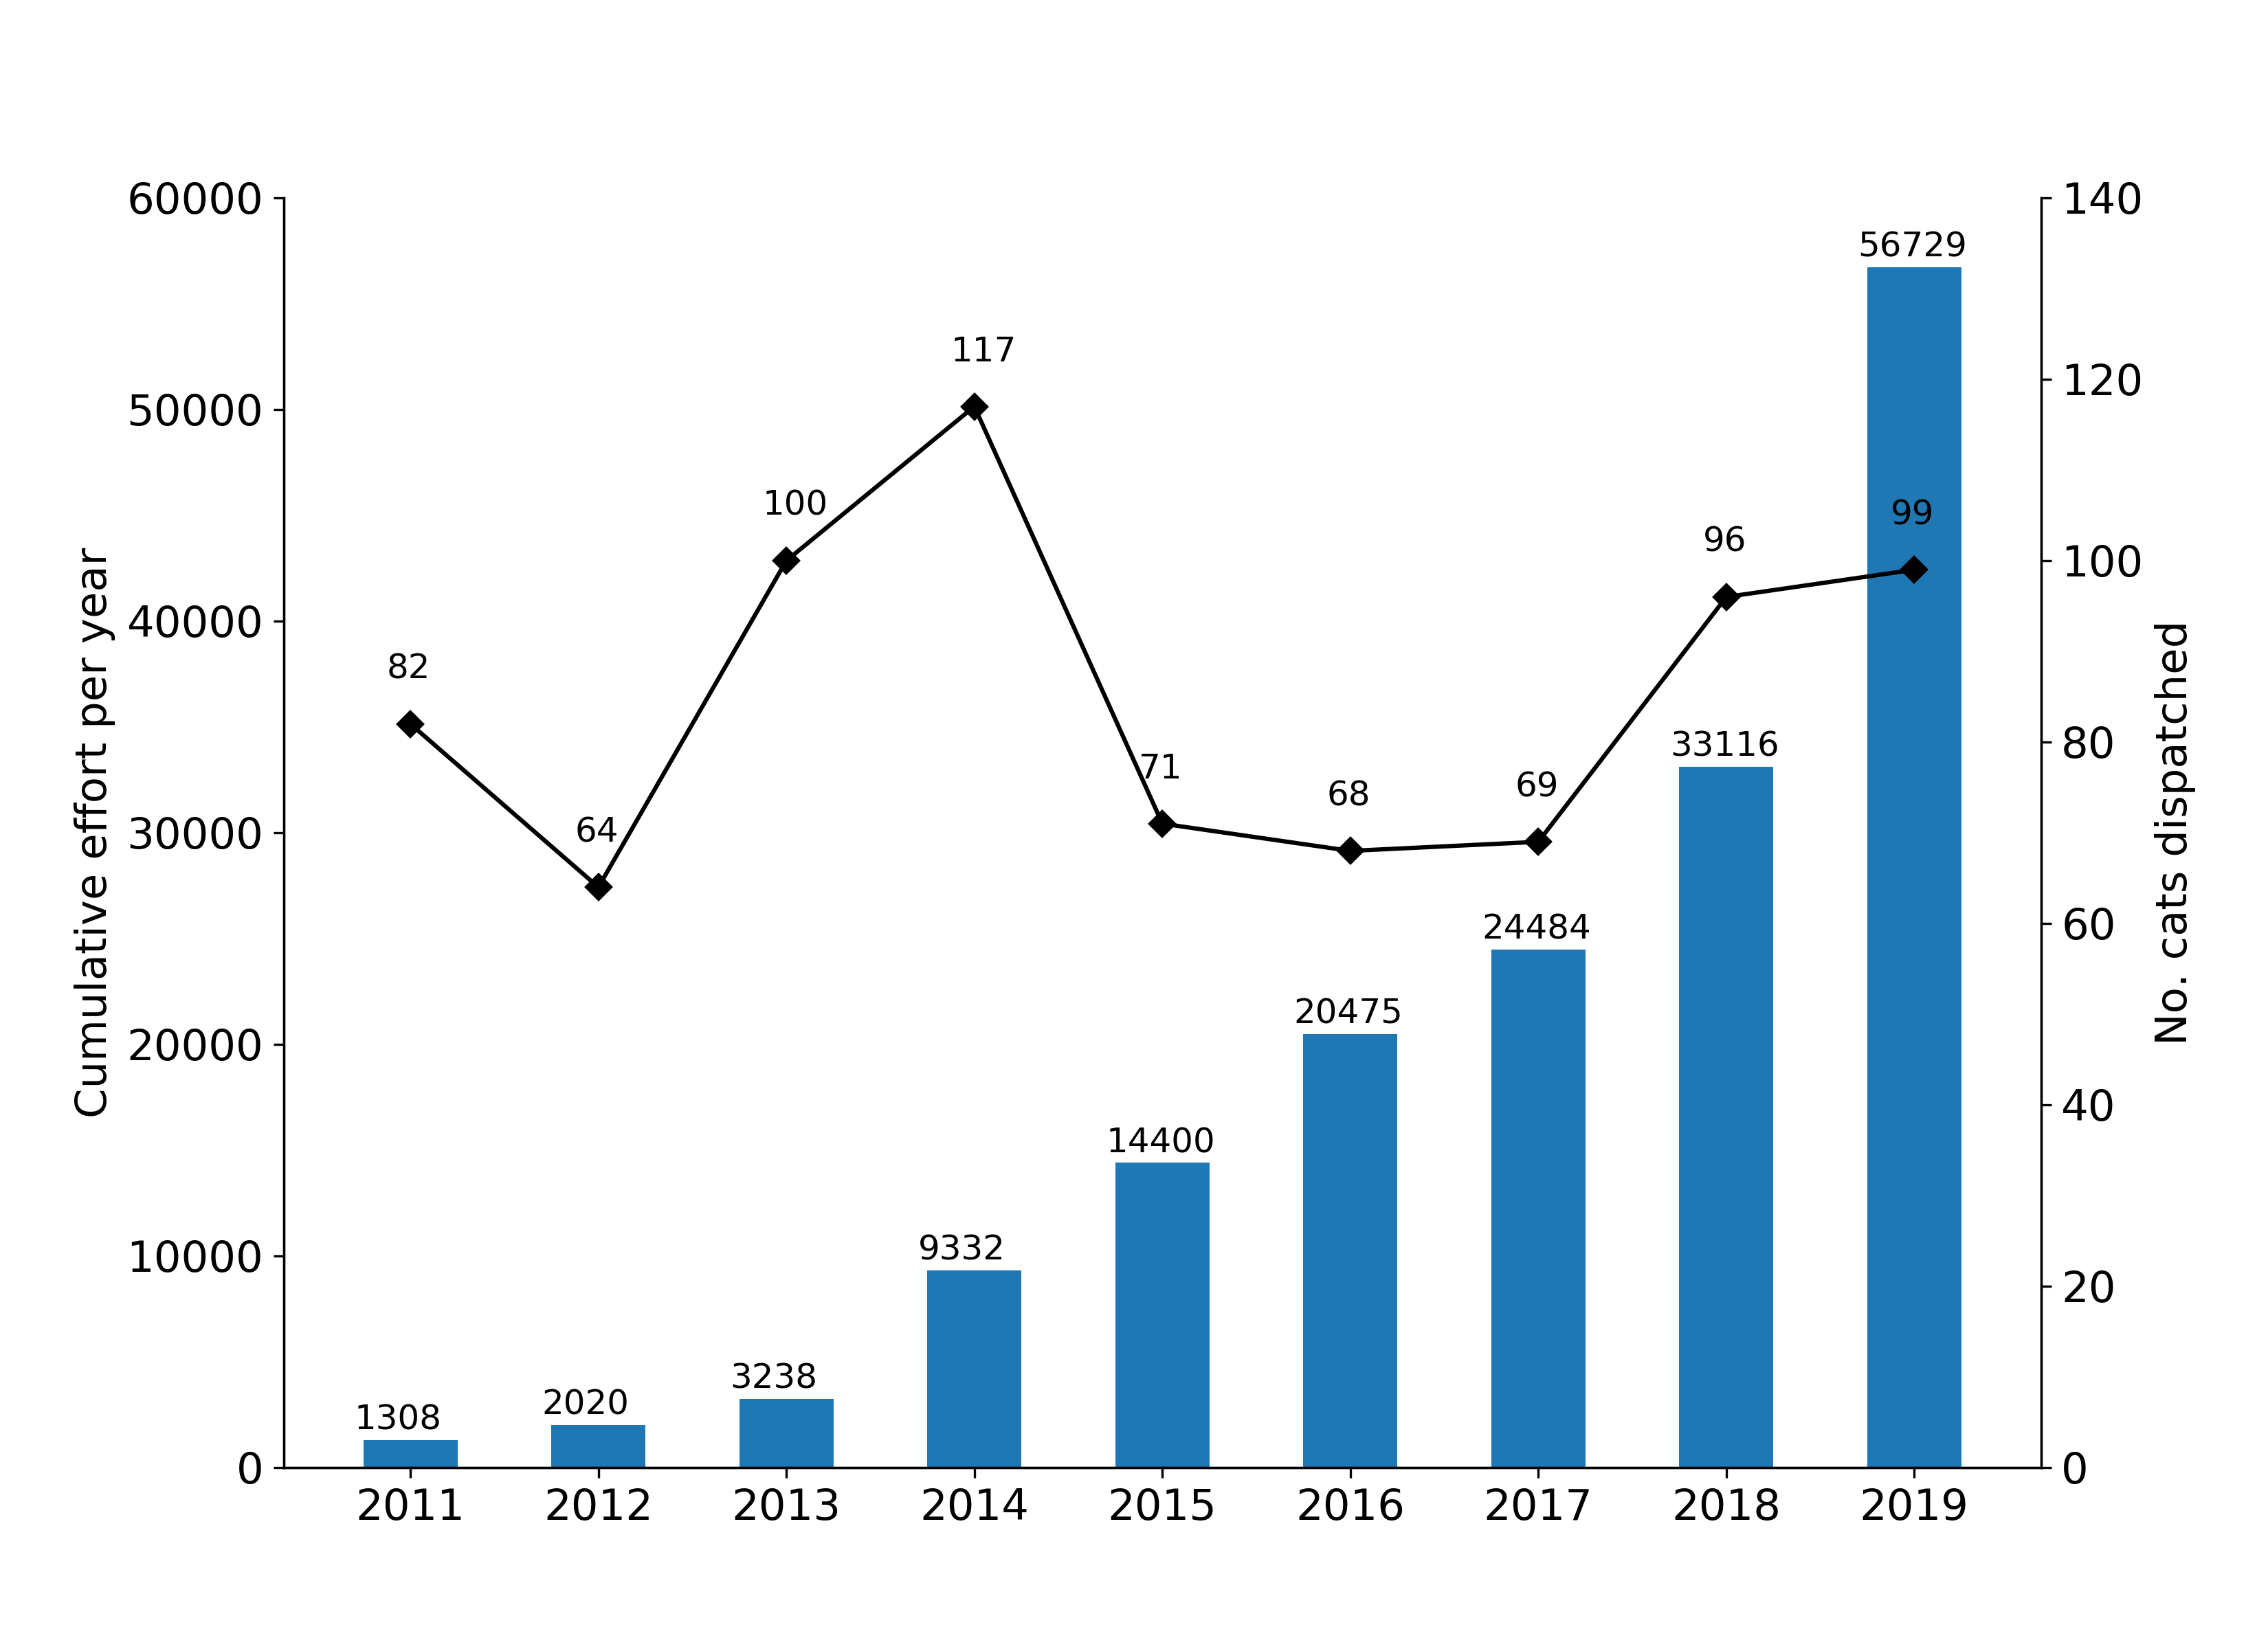
\includegraphics[scale=0.5]{figures/TotalCapturasPorAnioGatosSocorro.png}
\caption{Plot bar with the total effort (night-traps) per year.}
\label{fig:histogramaEsfuerzoTotalPorAnio}
\end{figure}


Table \ref{table:individuosRemanentes} shows: $\textnormal{P}_\textnormal{s}$, 
the amount of remaining individuals, and the $p$-value (level of trust) associated with the amount of remaining individuals.


\begin{table}[H]
\centering
\caption{\small{We show the probability of successful eradication ($\textnormal{P}_\textnormal{s}$), amount of remaining individuals and $p$-value associated with the amount of remaning cats.}}
\label{table:individuosRemanentes}
\begin{tabular}{ |c|c|c|c| }
    \hline
    Probability of & Remaining cats & $p$-value \\
    successful eradication ($\textnormal{P}_\textnormal{s}$) & & \\
    \hline
    0\%      & 76  & 0.581 \\
    \hline
\end{tabular}
\end{table}

\section*{Conclusion}

\begin{itemize}
\item To complete eradication by January 2020, an effort of 23900 night-traps each month must be applied. That means 27 trappers (with 30 traps each) need to be deployed
\item  TARGET: To complete eradication by July 2020, an effort of 9600 night-traps each month must be applied. That means 11 trappers (with 30 traps each) need to be deployed.
\item If current effort from the last expeditions is maintained (7825 night-traps), we will complete eradication in September 2020.
\end{itemize}

\section*{Referencias}

Ramsey, D. S., Parkes, J. P., Will, D., Hanson, C. C., and Campbell, K. J.
(2011). Quantifying the success of feral cat eradication, san nicolas island,
california. New Zealand Journal of Ecology, 35(2):163–173.
\end{document}
